Harmonic moments (or multipole moments) are defined for a collection of momenta $\vec{p}_i$, with respect to an axis $\vec{A}$ as \cite{Fox:1978vu}:
\begin{equation}
    B_l \equiv \sum_i \frac{|\vec{p}_i|}{\sqrt{s}}P_l(\cos\alpha_i),
\end{equation}
where $\sqrt{s}$ is the collision center-of-mass energy, $\alpha_i$ is the angle between the particles in the event and $\vec{A}$, and $P_l$ are Legendre polynomials.
In this analysis, the first 5 harmonic moments with respect to the thrust axis (see \Cref{sec:thrusts}) are considered.
The distributions for \textbf{Test~1} are shown in \Cref{fig:harmonicMomentumThrust0,fig:harmonicMomentumThrust1,fig:harmonicMomentumThrust2,fig:harmonicMomentumThrust3,fig:harmonicMomentumThrust4}.

\begin{figure}[htbp!]
    \subcaptionbox{\label{fig:harmonicMomentumThrust0}}{
        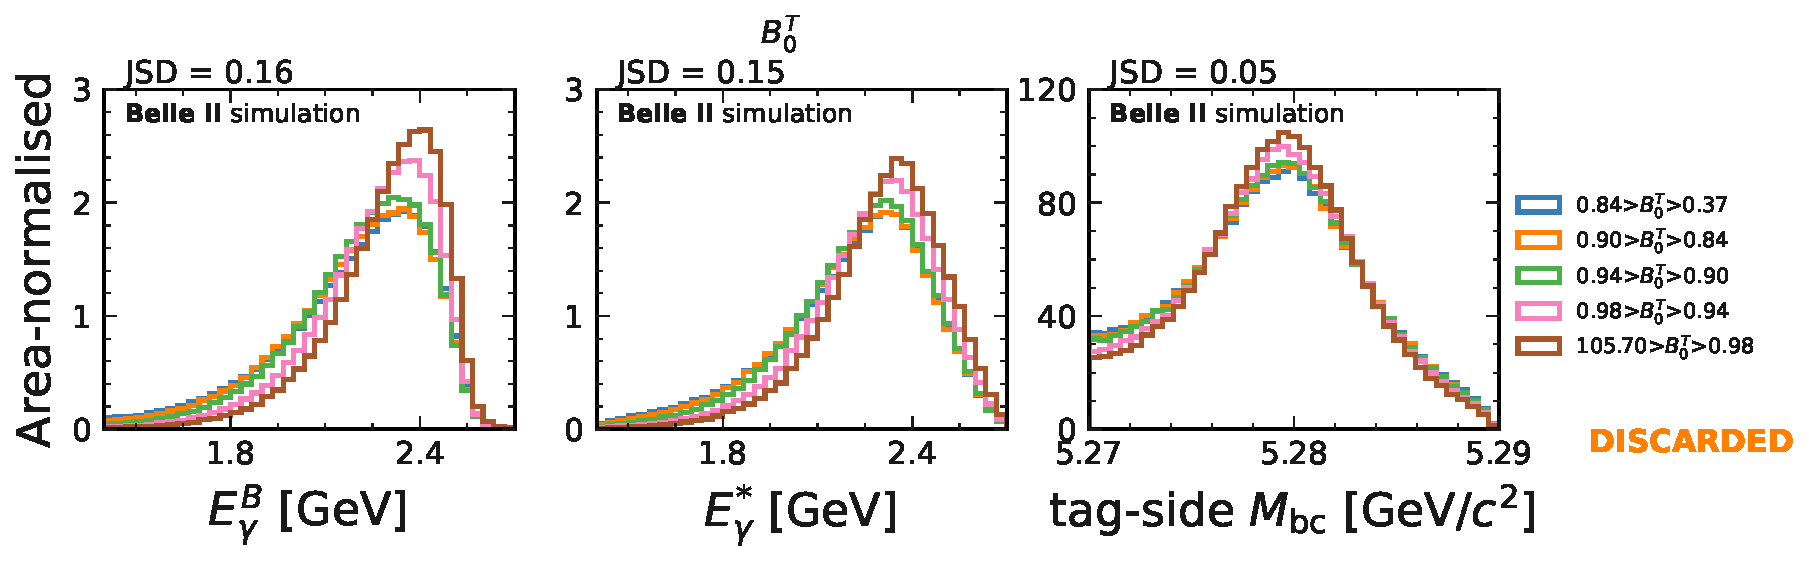
\includegraphics[width=0.95\textwidth]{figures/appendices/continuum_suppression_features/harmonic_moments/harmonicMomentThrust0_bias_tested.pdf}
    }
    \subcaptionbox{\label{fig:harmonicMomentumThrust1}}{
        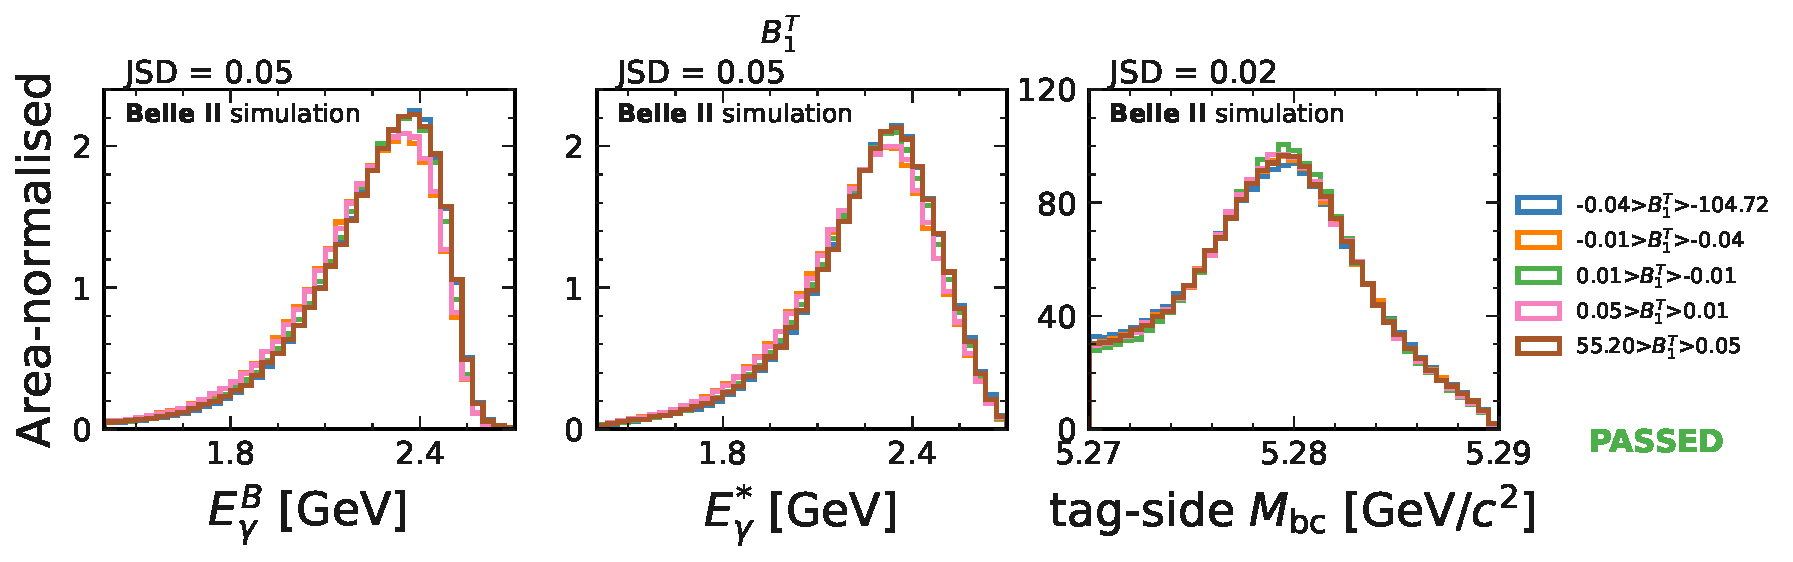
\includegraphics[width=0.95\textwidth]{figures/appendices/continuum_suppression_features/harmonic_moments/harmonicMomentThrust1_bias_tested.pdf}

    }
\end{figure}
\begin{figure}[htbp!]
    \ContinuedFloat
    \subcaptionbox{\label{fig:harmonicMomentumThrust2}}{
        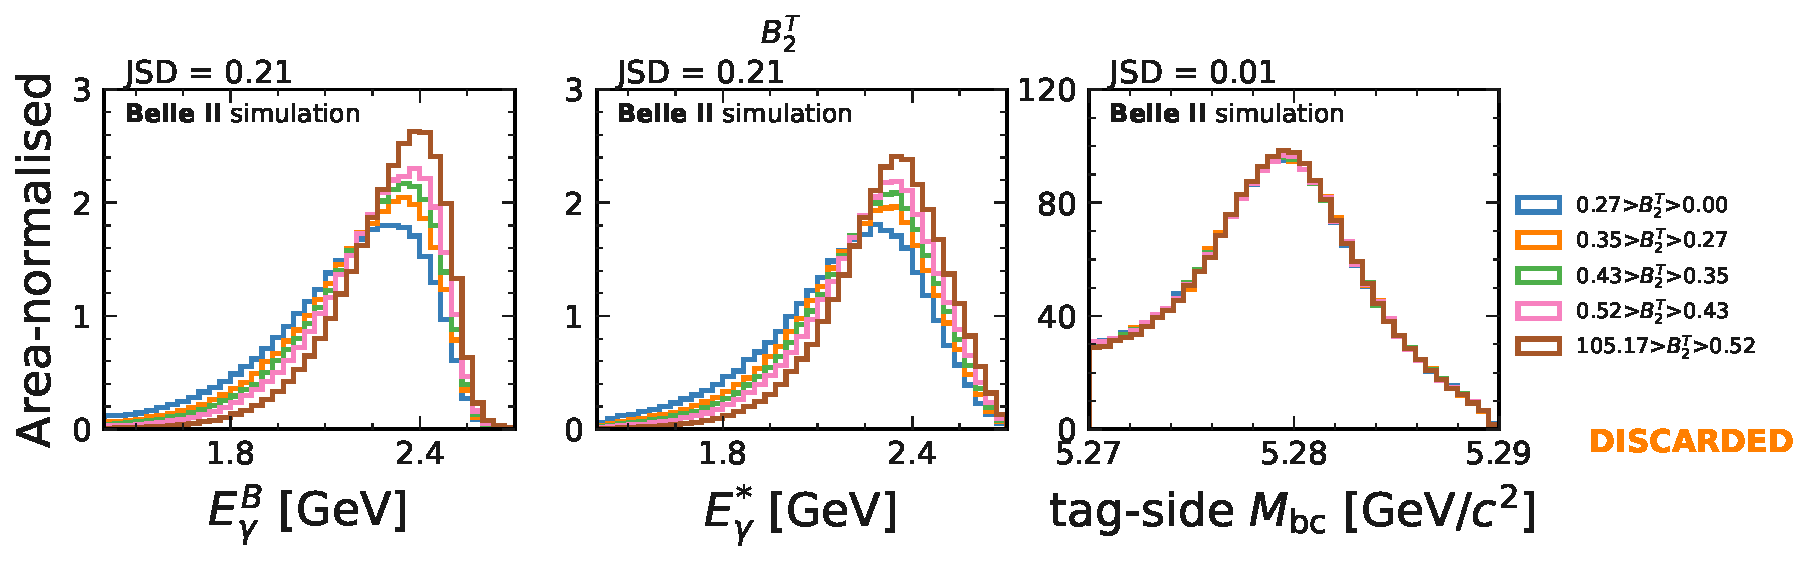
\includegraphics[width=0.95\textwidth]{figures/appendices/continuum_suppression_features/harmonic_moments/harmonicMomentThrust2_bias_tested.pdf}

    }
    \subcaptionbox{\label{fig:harmonicMomentumThrust3}}{
        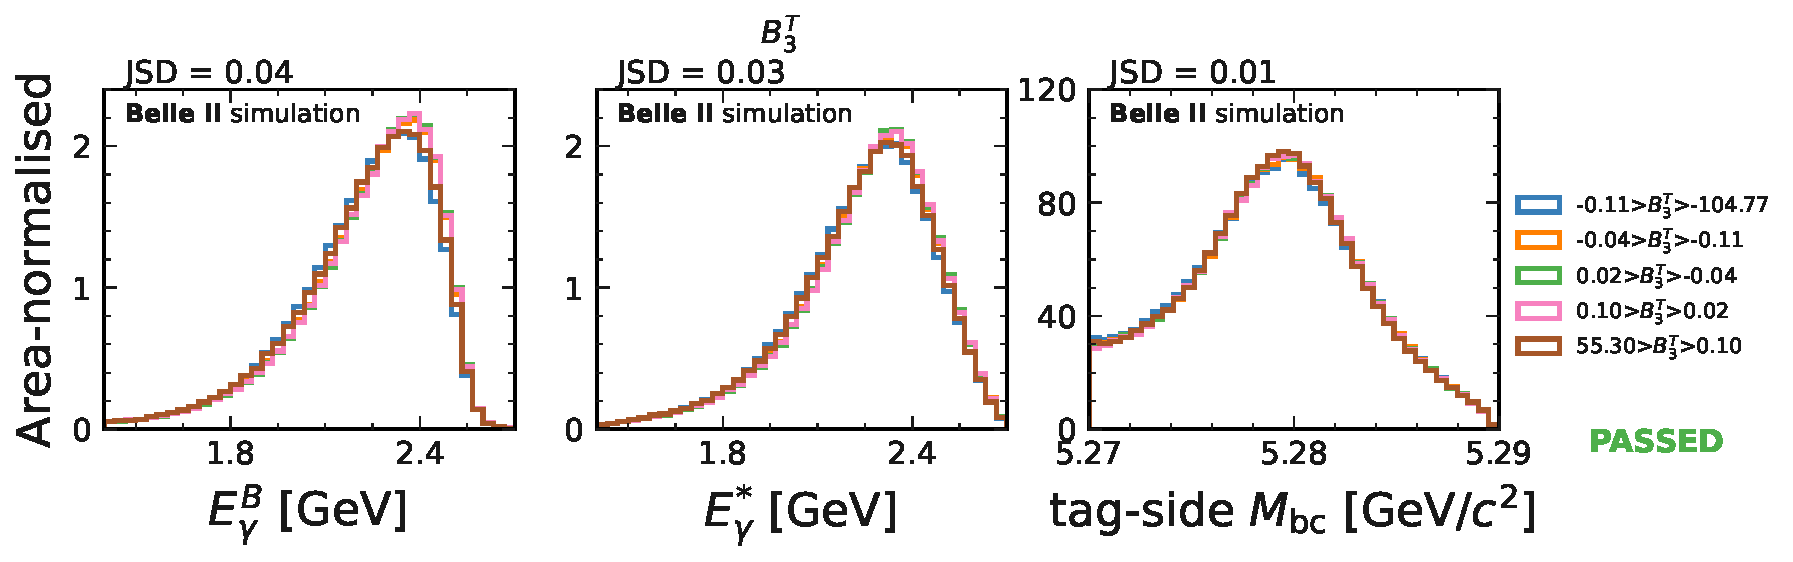
\includegraphics[width=0.95\textwidth]{figures/appendices/continuum_suppression_features/harmonic_moments/harmonicMomentThrust3_bias_tested.pdf}

    }
    \subcaptionbox{\label{fig:harmonicMomentumThrust4}}{
        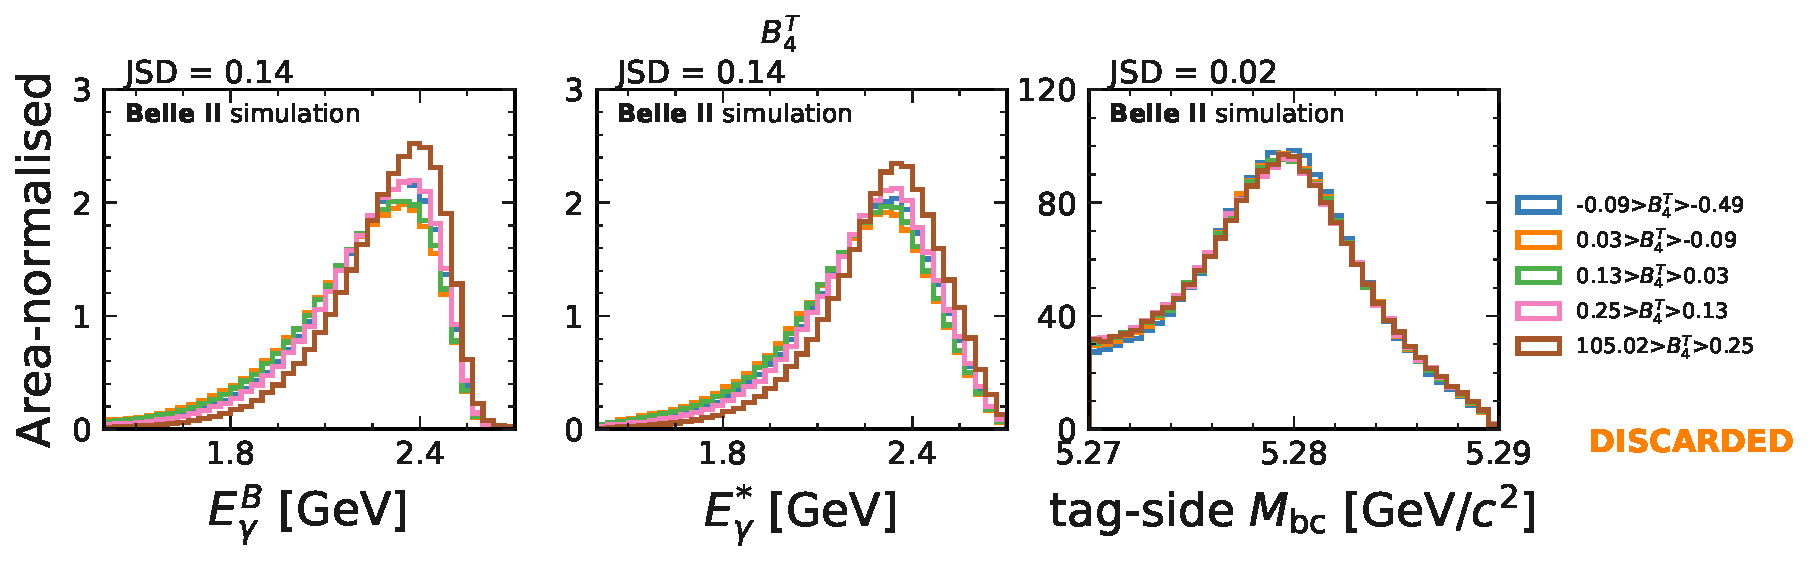
\includegraphics[width=0.95\textwidth]{figures/appendices/continuum_suppression_features/harmonic_moments/harmonicMomentThrust4_bias_tested.pdf}
    }

    \caption{\label{fig:harmonicmoments_test1} The bias-test on \EB, \Estar and \Mbc for harmonic thrust observables.
    The test is performed based on \textbf{Test~1} strategy, defined in \Cref{sec:continuum_features}.
    Variable definitions are given in the text.}
\end{figure}
